% !TEX root = ../main.tex
\subsection{Deep Inelastic Scattering} \label{sec::dis}
% --+ Basic description +-------------------------------------------------------
    In its simplest description, Deep Inelastic Scattering (DIS) is the scattering of an electron off a quark inside a nucleon.
    Figure \ref{fig::dis_diagram} shows the Feynman diagram of DIS.
    The four-momentum of the nucleon is $P$, that of the quark is $p$, and the initial and final four-momenta of the electron are $k$ and $k'$, respectively.
    If $k'$ is measured, then the momentum transferred to the hadron system by the virtual photon is $q = k - k'$.
    $q$ is a spacelike vector, conventionally denoted as $q^2 = -Q^2$.

    \begin{figure}[h!]
        \centering\frame{
        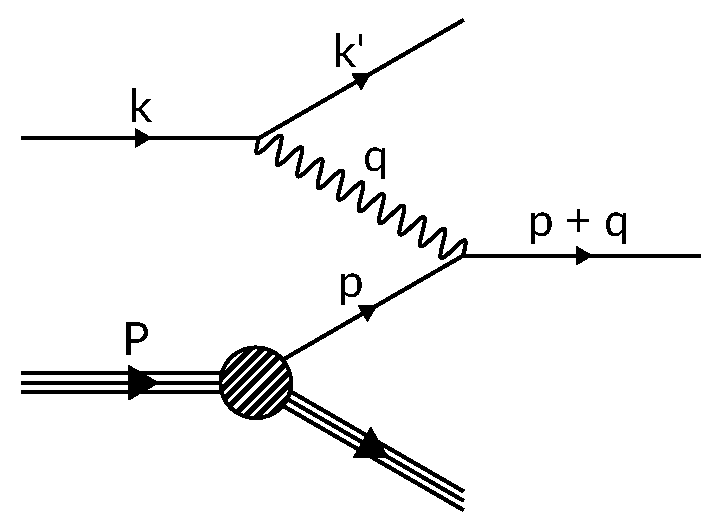
\includegraphics[width=0.6\textwidth]{10physicsmotivation/img/10dis_diagram.pdf}}
        \caption[DIS in QCD.]{DIS in QCD. The diagram describes the stream of momentum in the scattering of a high energy electron off a quark. The quark's wave function is incorporated in the nucleon's wave function. Source: Own elaboration.}
        \label{fig::dis_diagram}
    \end{figure}

    If $Q^2$ is high enough, the quark is knocked out of the nucleon.
    Soft processes like gluon emission and quark-antiquark pair production then occur to neutralise the colour.
    This transforms the knocked-out quark into a jet of hadrons.
    This jet propagates in the direction of the electron's transferred momentum.

% --+ Approximating the cross section +-----------------------------------------
    To approximate the cross section of the electron-nucleon scattering, we'll work on the center of mass reference frame.
    Here, the electron and nucleon are propagating towards each other with enough energy to let us ignore the mass of the latter.
    Due to this, the nucleon has almost lightlike momentum along the collision axis.
    Its constituent quarks must therefore also have lightlike momenta, almost collinear to the nucleon's.
    Hence, to first order approximation, we can say of the quark's momentum is
    \begin{equation*}
        p = \xi P,
    \end{equation*}
    where $\xi$ is the longitudinal fraction of the quark's momentum, and as such $0 < \xi < 1$.

    In leading order approximation, we can also ignore the gluon emission and exchange during the collision.
    Then, the cross section of the electron-nucleon scattering is equal to that of the electron-quark's for a given $\xi$, multiplied by the probability that the nucleon contains a quark with $\xi$ longitudinal momentum fraction, integrated over $\xi$.

    This calculation has the problem that the probability that the nucleon contains a quark with a particular momentum can't be calculated in perturbative QCD.
    It depends on the soft processes that define the structure of the nucleon as a bound state of quarks and gluons.
    We must therefore consider this probability an unknown function to be measured in the experiment.

    This kind of probability functions are called Parton Distribution Functions (PDF).
    A PDF can be used for all kinds of quarks, antiquarks, and gluons, and are incorporated inside the nucleon's wave function.
    For each parton $f$, its PDF is defined as
    \begin{equation*}
        P_f = f_f(\xi)d\xi.
    \end{equation*}
    Therefore, the cross section of the inelastic scattering of the electron off the nucleon in leading order approximation is
    \begin{equation*}
        \sigma\left( e^-(k) p(P) \rightarrow e^-(k') X \right) =
                \int_0^1d\xi \sum_f f_f(\xi) \cdot
                \sigma\left( e^-(k) q_f(\xi P) \rightarrow e^-(k') + q_f(p') \right)
    \end{equation*}
    where $X$ indicates the final hadronic state.
    One should remember that this equation is not an exact QCD prediction, but is the first-term expansion of $\alpha_s$.
    This approximation is the parton model \cite{halzen1991}.

% --+ The parton model +--------------------------------------------------------
    \begin{figure}[b!] % NOTE. Figure out source.
        \centering\frame{
        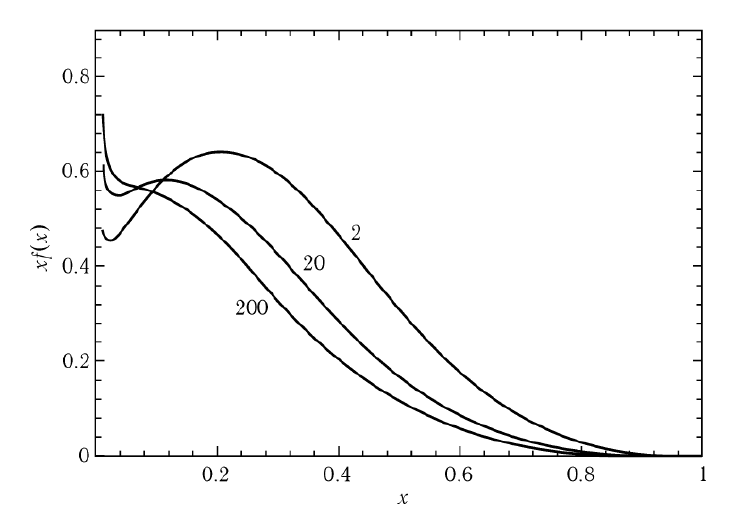
\includegraphics[width=0.8\textwidth]{10physicsmotivation/img/10q2_dependence_u.png}}
        \caption[$Q^2$ dependence of $x$ PDF for the $u$ quark.]{$xf_f(x)$ parton distribution functions for the $u$ quark when $Q = 2$, $Q = 20$, and $Q = 200$ GeV.
        The plots show the parton evolution effect according to the Altarelli-Parisi equations.}
        \label{fig::q2dependenceu}
    \end{figure}

    In the parton model, the cross section is
    \begin{equation}
        \label{eq::parton_model_cross_section}
        \frac{d^2\sigma}{dxdy} \left( e^-p \rightarrow e^-X \right) =
                \left( \sum_f xf_f \left( x, Q^2 \right) Q_f^2 \right)
                \frac{2\pi\alpha s}{Q^4} \left( 1 + \left( 1 - y \right)^2 \right),
    \end{equation}
    where $s \equiv 2P\cdot k$, $Q_f$ is the charge of the parton $f$, and $x$ and $y$ are the Bjorken variables, defined as
    \begin{equation*}
        x \equiv \frac{Q^2}{2P\cdot q}, \hspace{36pt} y \equiv \frac{2 P\cdot q}{s}.
    \end{equation*}
    In the nucleon's rest frame, $y = q^0/k^0$, and thus it is the energy transferred to the hadron by the incoming electron.

    Due to gluon radiation, the PDFs in equation \eqref{eq::parton_model_cross_section} have a weak dependence on $Q^2$.
    This leads to Bjorken scaling violation \cite{halzen1991}.
    When the structure functions are known for certain values of $Q^2$, they can be evolved to other values using the Dokshitser-Gribox-Lipatov-Altarelli-Parisi (DGLAP) equations \cite{dokshitzer1991}.

    Figure \ref{fig::q2dependenceu} shows the predictions of the Altarelli-Parisi equations for the evolution of the PDFs dependence on $Q^2$.
    Partons with large $x$ tend to radiate and move to states with lower $x$.
    Parallel to this, the radiations produce new partons with low $x$ values.
    With an increase in $Q^2$, the parton distributions decrease for large $x$ values, while quickly increasing for low $x$.
    At low $Q^2$, the wavelength of the virtual photon is too large to probe the partons, thus probing the proton as a whole.
    The validity range for the QCD-extended parton model is not precisely known, but is assumed to be valid for $Q^2 > 1 \text{ GeV}^2$, corresponding to a spatial resolution of about $0.2$ fm.

% --+ Strong Coupling Constant +------------------------------------------------
    \subsubsection{Strong Coupling Constant $\alpha_s$}
        Measuring the experimental value of $\alpha_s$ is important for perturbative QCD calculations.
        To do this, one should determine the overall scale of renormalisation.
        This is usually selected to be the mass of the neutral Bose particle $Z^0$, which is $91.19$ GeV.
        Additionally, one should fix the scheme of renormalisation, which defines the coupling constant in a given scale.
        The experimental results for $\alpha_s$ can be seen on figure

        \begin{figure}[b!] % NOTE. Figure out source.
            \centering\frame{
            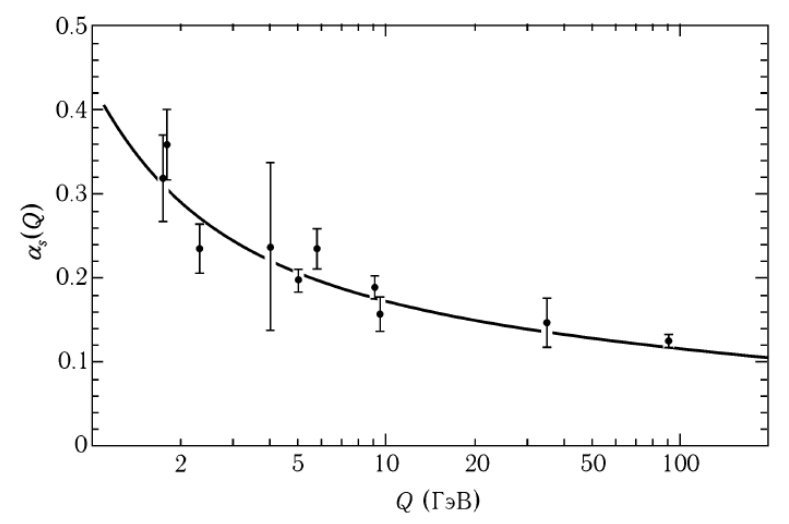
\includegraphics[width=0.8\textwidth]{10physicsmotivation/img/11strong_coupling_constant_q.png}}
            \caption[$\alpha_s$ dependence on $Q^2$.]{Experimentally measured $\alpha_s$ dependence on $Q$.
            The measured values are compared with theoretical predictions of renormalised evolution with initial $\alpha_s(m_z) = 0.117$ GeV.}
            \label{fig::alpha_q_dependence}
        \end{figure}
